\begin{ZhChapter}

    \chapter{Implementation}
    \section{Experimental Setup}
    The experimental implementation of this study was conducted on the Windows 11 operating system. Visual Studio Code (VS Code) was utilized as the primary development environment, integrated with the Anaconda distribution for Python to manage package dependencies and virtual environments. A range of scientific computing and machine learning packages were installed to facilitate algorithm development, model training, and evaluation workflows. Detailed configuration steps and setup instructions are described in the following subsection.

    \subsection{Hardware Requirements}

    Table \ref{table:hardware} provides detailed specifications and purposes of each hardware component utilized in our experimental environment.

    \begin{table}[htbp]
        \centering
        \caption{Hardware Requirements}
        \label{table:hardware}
        \begin{tabular}{|l|l|}
            \hline
            \textbf{Component} & \textbf{Specification}                            \\ \hline
            CPU                & 12th Gen Intel(R) Core(TM) i5-12500H @ 2.50 GHz   \\ \hline
            RAM                & 16.0 GB (15.6 GB usable)                          \\ \hline
            Storage            & Built-in SSD (operating system and model storage) \\ \hline
        \end{tabular}
    \end{table}

    \subsection{Software Requirements}

    Table \ref{tab:software} lists the software used in our experimental setup, along with their purposes and license types.

    \begin{table}[htbp]
        \centering
        \caption{Software and Libraries Used in the Experiment}
        \label{tab:software}
        \begin{tabular}{|l|c|p{7cm}|c|}
            \hline
            \textbf{Software}                & \textbf{Version} & \textbf{Purpose}                                                                                                                                                 & \textbf{License} \\ \hline
            Visual Studio Code~\cite{vscode} & 1.89.1           & A lightweight and extensible code editor used as the primary integrated development environment (IDE) for editing Python scripts and managing project structure. & MIT              \\ \hline
            Anaconda Prompt~\cite{anaconda}  & 2024.02          & A command-line interface provided by the Anaconda distribution, used for managing Python virtual environments and installing dependencies via Conda or pip.      & BSD              \\ \hline
            Python~\cite{python}             & 3.9.18           & The main programming language used to implement the core modules of the proposed system, including preprocessing, model training, and evaluation routines.       & Python License   \\ \hline
            NumPy~\cite{numpy}               & 1.26.4           & Provides high-performance array structures and functions for numerical computing, especially efficient vector and matrix operations.                             & BSD              \\ \hline
            Pandas~\cite{pandas}             & 2.2.2            & Offers powerful data manipulation and analysis tools, including DataFrame structures used for preprocessing and filtering packet data.                           & BSD              \\ \hline
            Scikit-learn~\cite{scikit-learn} & 1.4.2            & Provides a wide range of machine learning algorithms, particularly the Multi-Layer Perceptron (MLP) classifier used in this study.                               & BSD              \\ \hline
            mmh3~\cite{mmh3}                 & 4.0.1            & Implements MurmurHash3, a fast non-cryptographic hashing function used to convert tokens into integer values for embedding.                                      & MIT              \\ \hline
            PyTorch~\cite{torch}             & 2.2.2+cpu        & A deep learning framework used to define and train neural networks, including custom embedding and classification models.                                        & BSD              \\ \hline
        \end{tabular}
    \end{table}



    \subsubsection{Environment Setup}

    \textbf{Step 1: Installing Anaconda}

    Anaconda is an open source Python platform designed for data science and machine learning development, integrating the most commonly used data analysis tools and libraries. It has a rich built-in data science suite, including core tools such as Numpy (numerical operations), Pandas (data processing), and Seaborn (data visualization).\footnote{https://www.anaconda.com/products/distribution}

    Go to the official Anaconda website (figure \ref{fig: DownloadAnaconda}) and select the appropriate operating system version (Windows, macOS or Linux).
    According to the system recommendations of your computer, choose the 64-bit version for better performance.
    \begin{figure*}[htbp]
        \centering
        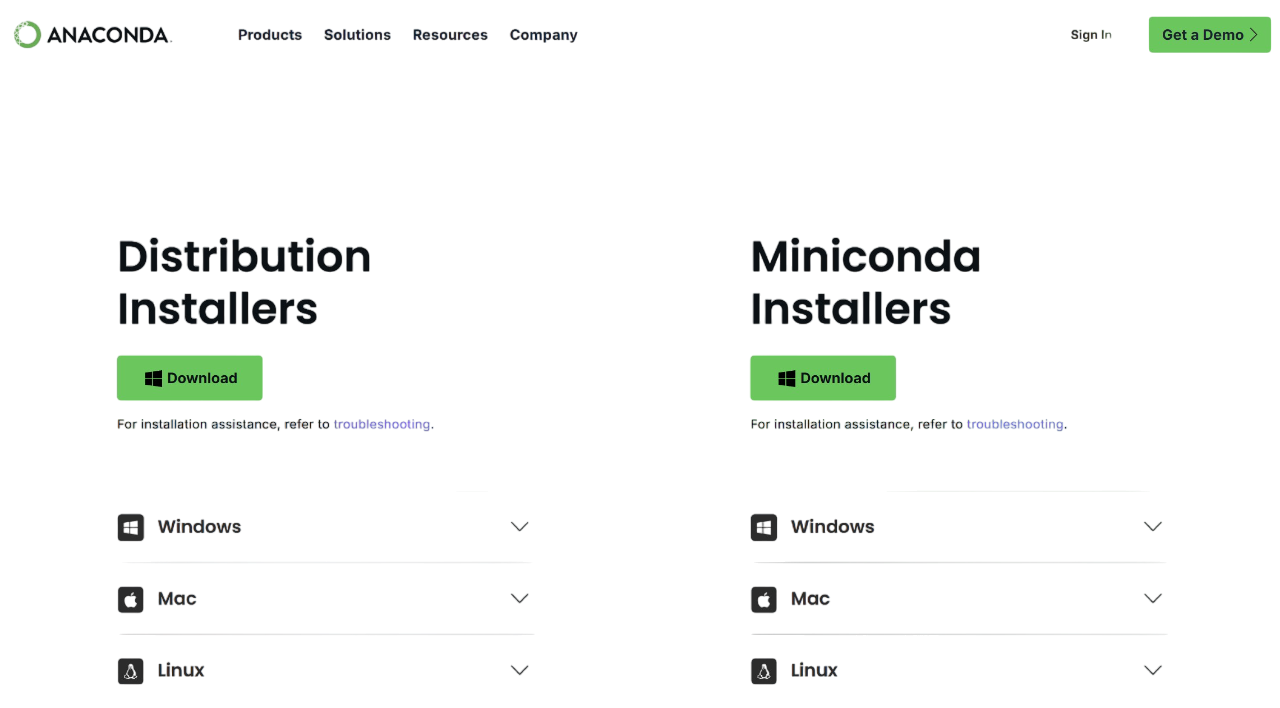
\includegraphics[width = 0.5\textwidth]{image/DownloadAnaconda.jpg}
        \caption{Download on Official Anaconda Website}
        \label{fig: DownloadAnaconda}
    \end{figure*}

    Install Anaconda
    Double-click the downloaded Anaconda installation file (installer) to start the installation program. And click "Next" to proceed to the next step (\ref{fig: InstallAnaconda}).
    Select the installation type. If it is for personal use only, it is recommended to select "Just Me", then click "Next".
    \begin{figure*}[htbp]
        \centering
        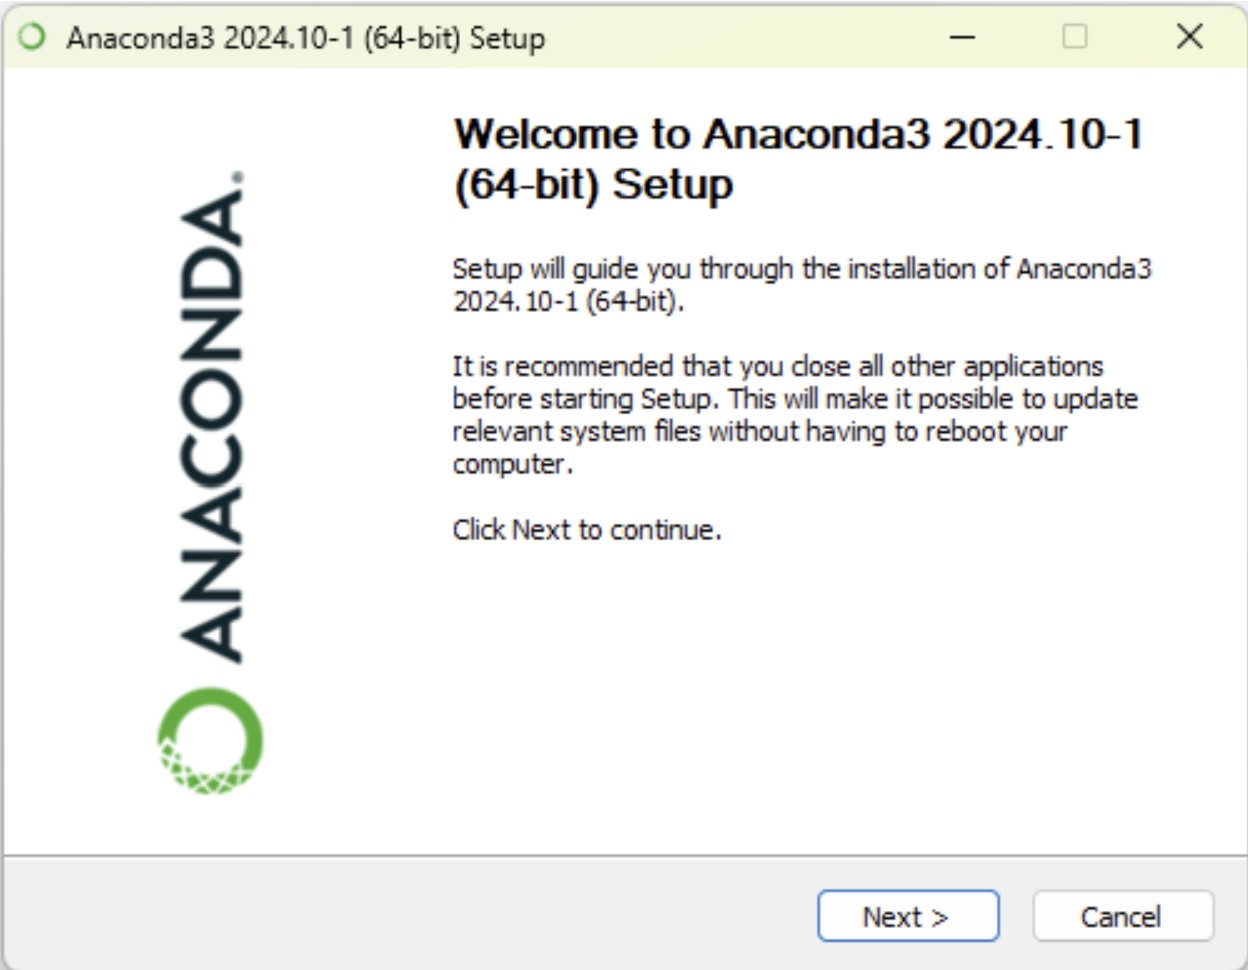
\includegraphics[width = 0.5\textwidth]{image/InstallAnaconda.jpg}
        \caption{Installation for Anaconda}
        \label{fig: InstallAnaconda}
    \end{figure*}

    In the installation options, it is recommended not to check Add Anaconda to the PATH environment variable (unless there are special requirements), and directly click "Install" to start the installation.

    Once the installation is complete, find and launch Anaconda Navigator from the Windows Start menu (figure \ref{fig: AnacondaMenu}).
    \begin{figure*}[htbp]
        \centering
        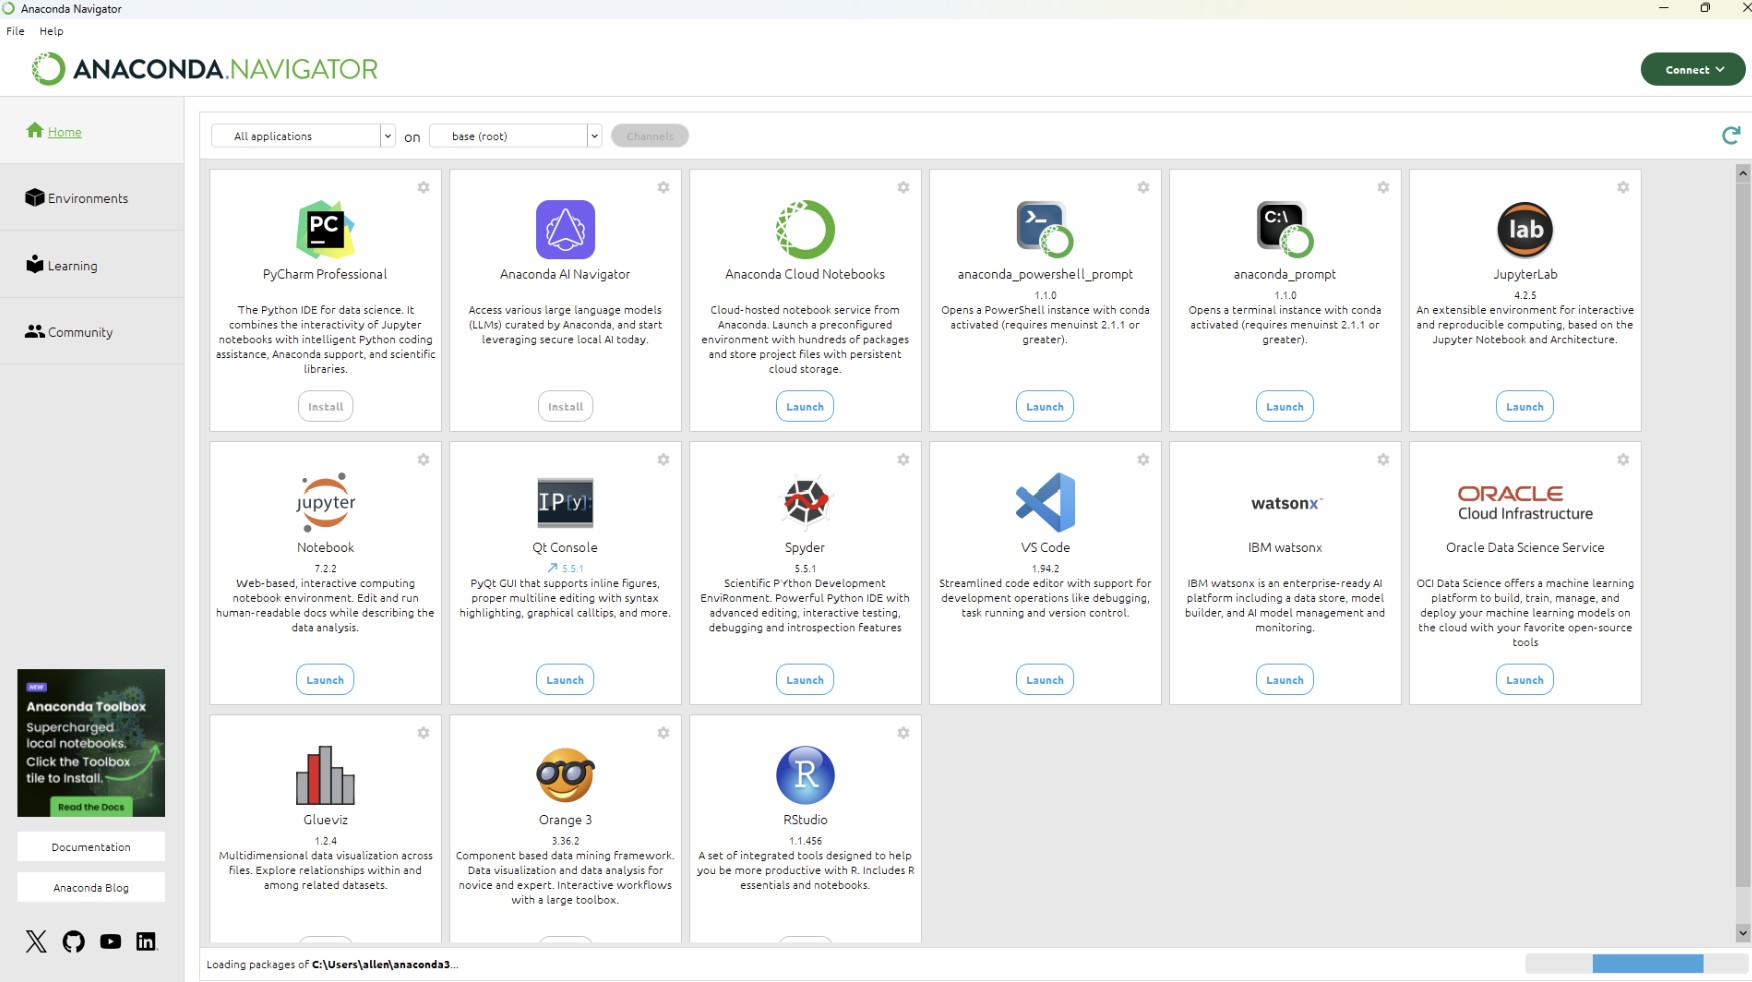
\includegraphics[width = 0.5\textwidth]{image/AnacondaMenu.jpg}
        \caption{FlowChart for Preprocess Model}
        \label{fig: AnacondaMenu}
    \end{figure*}




    \textbf{Step 2: Installing Visual Studio Code}

    Visual Studio Code (VS Code) (figure \ref{fig: VS}) is a lightweight and extensible source code editor that, when used with the Python Extension, offers enhanced development capabilities. The installation package can be obtained from the official website\footnote{https://code.visualstudio.com/}.

    \begin{figure*}[htbp]
        \centering
        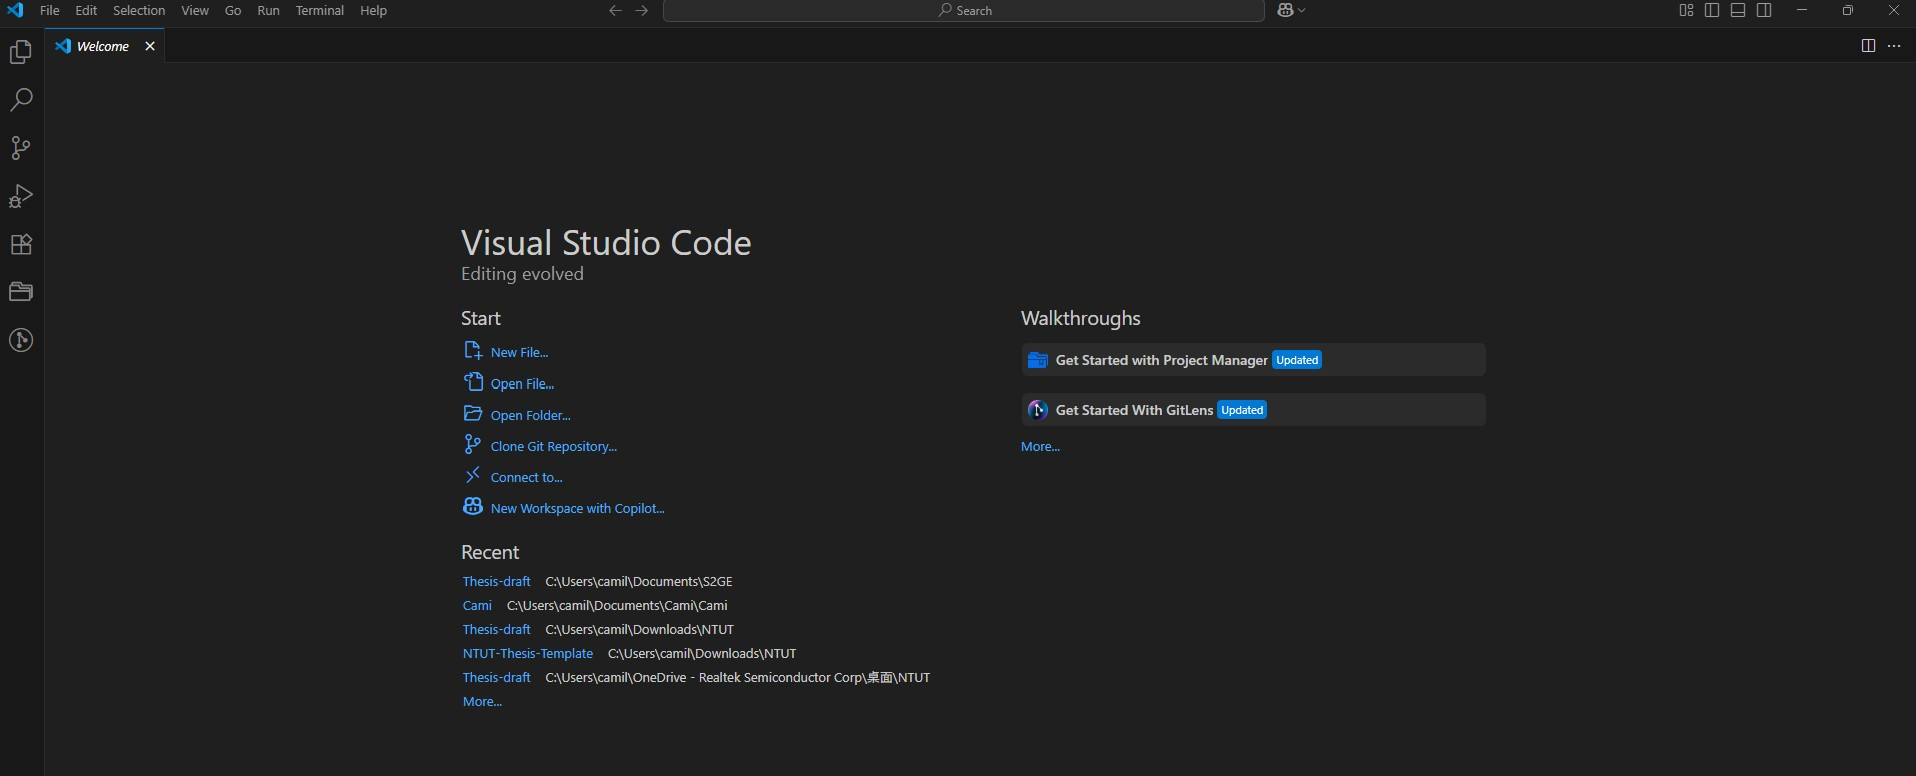
\includegraphics[width = 0.5\textwidth]{image/VS.jpg}
        \caption{Visual Studio Code}
        \label{fig: VS}
    \end{figure*}

    \subsubsection{Creating Virtual Environment and Installing Packages}

    \textbf{Step 3: Creating a Python Virtual Environment}

    Use the Anaconda Prompt to create a virtual environment with the designated Python version:
    \begin{verbatim}
    conda create -n nids_env python=3.9
    conda activate nids_env
    \end{verbatim}

    \textbf{Step 4: Installing Required Packages}

    The packages required in this study are listed below and can be installed using pip:
    \begin{verbatim}
    pip install numpy pandas scikit-learn matplotlib seaborn torch mmh3
    \end{verbatim}
    A brief description of each package is provided in Table~\ref{tab:software}.


    \textbf{Step 5: Selecting the VS Code Interpreter}

    In Visual Studio Code, press \texttt{Ctrl+Shift+P} to open the command palette, then select \textit{"Python: Select Interpreter"}. Choose the previously created \texttt{nids\_env} virtual environment from the list of available interpreters.

    \subsubsection{4.1.4 Verifying the Installation}

    To verify the installation, create a file named \texttt{main.py} and include the following test code:
    \begin{verbatim}
    import numpy as np
    import pandas as pd
    import torch
    import mmh3
    print("All packages loaded successfully!")
    \end{verbatim}

    Execute the script in the terminal with the following command:
    \begin{verbatim}
    python main.py
    \end{verbatim}

    If the message is displayed successfully, it indicates that the environment has been set up correctly.






\end{ZhChapter}